\chapter{Inter-Vehicles}

\section{Global Positioning System}
The \textbf{\textit{GPS}} in origin named \textbf{NAVigation Satellite Timing and Ranging Global Positioning System} (\textbf{NAVSTAR GPS}) is one of the space-based \textit{global navigation satellite system} (\textbf{GNSS}) that provides \textbf{geolocation} and \textbf{time information} anywhere on the Earth, using the signal of at least four satellite. The geolocation information gives an \textbf{XYZ} coordinates.

\subsection{Actors}
\textbf{GPS} is based on three elements: \textbf{space segment} (the satellite), \textbf{control segment} (ground station) and \textbf{user segment} (end-user equipments):
\begin{enumerate}[nosep]
    \item \textbf{space segment}: have the main goal to broadcast navigation message constantly.
    \item \textbf{control segment}: ground antennas that \textit{track}, \textit{collect} and \textit{correct} all the \textbf{sat orbits} (normally they are very precise and known a priory). They both recive/transmit data from/to satellites.
    \item \textbf{user segment}: cheap devices used to collect GPS signal and know the position (it has the maximum error approximately of 1 meter).
\end{enumerate}

\subsection{NAV Msg}
The information \textbf{broadcasted} by the satellite is called \textbf{\textit{Navigation Message}} (\textbf{NAV}). The nav msg is composed by:
\begin{figure}[h]
    \centering
    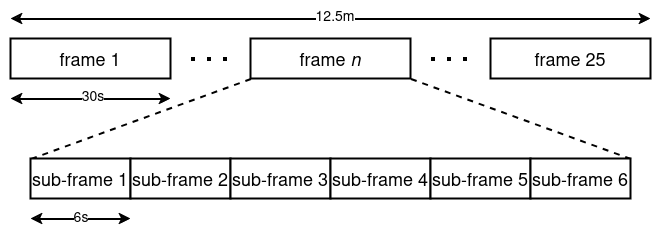
\includegraphics[width=0.75\textwidth]{img/gps_frame}
\end{figure}
\begin{itemize}[nosep]
    \item \textbf{25 frames} (or \textbf{pages}) that takes 12.5 minutes to be transmitted.
    \item each frame takes 30 seconds to be transmitted and it is formed by \textbf{6 sub-frame}.
    \begin{enumerate}[nosep]
        \item the first sub-frame contains the \textbf{satellite clock information}.
        \item the second and the third give the information about the \textbf{satellite ephemeris} (\textbf{orbit}).
        \item the forth and thr fifth are different and are complete only receiving all the 25 frames of the NAV msg, they have the \textbf{Almanac \& constellation status}.
    \end{enumerate}
    \item each sub-frame needs 6 seconds to be transmitted, and it is composed by \textbf{10 words}.
    \item each word consist of \textbf{30 bits} and it takes 0.6 second to be transmitted.
\end{itemize}

\newpage
\subsection{Bit Coding}
GPS use the \textbf{Bi-Phase Shift Key} (\textbf{BPSK}) modulation technique. In BPSK the carrier signal is modified by altering its phase by 180 degree, for each symbol. A phase shift of 180 degrees denotes a binary 0 while no phase shift represents a binary 1. The advantages to use this type of mudaltion technique is:
\begin{enumerate}[nosep]
    \item rendundancy
    \item jamming resistance
    \item measure \& remove the ionospheric delay
    \item requires a dual frequency receiver (with a single one it is possible to survive but less accuracy) one at $1575.42MHz$ and the other one at $1227.60MHz$.
\end{enumerate}
\begin{figure}[h]
    \centering
    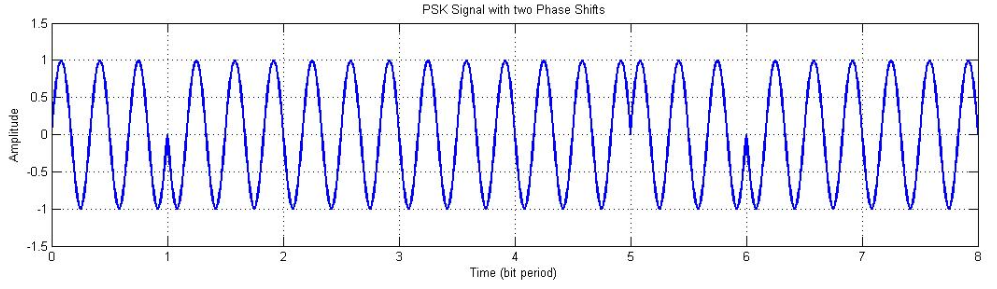
\includegraphics[width=\textwidth]{img/bspk_wave}
\end{figure}
\begin{figure}[h]
    \centering
    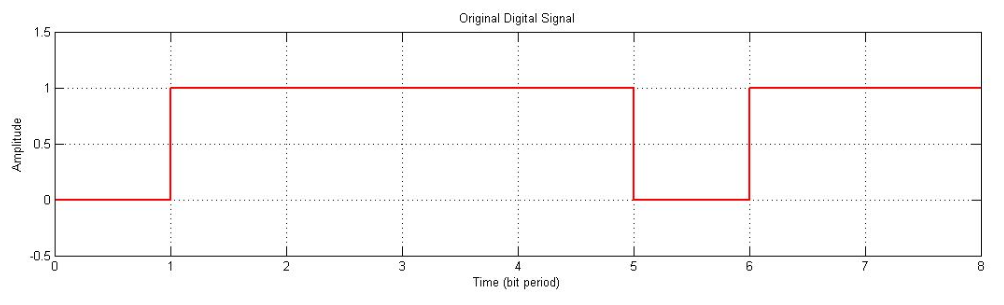
\includegraphics[width=\textwidth]{img/bspk_signal}
\end{figure}

\newpage
\subsection{Working Principle}
Let's distinguish the study of the working principle in two hypotheses: \textbf{theoretical}: receiver clock is perfectly synchronize with the satellite clock (\textit{absolute clock}); and \textbf{reality}: receiver clock is cheap, non-atomic and not perfectly synchronize with the satellite clock.

\begin{figure}[h]
    \centering 
    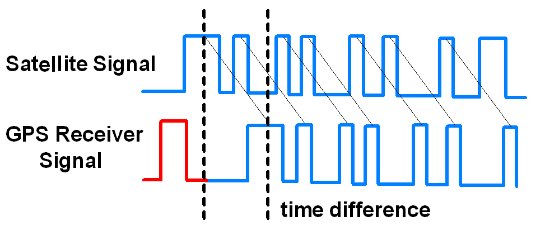
\includegraphics[width=0.45\textwidth]{img/hp_theory}
    \caption{Satellite-Receiver clock synch}
\end{figure}
In the first hypothesis, we know: \textbf{satellite position} (written in the NAV), \textbf{satellite clock} (written in the NAV) and the \textbf{speed of light} $c$. So it is possible to obtain:
\begin{enumerate}[nosep]
    \item \textbf{signal travel time}: $\Delta t = clock_{recv} - clock_{NAV}$
    \item \textbf{distance satellite-receiver}: $d = c \cdot \Delta t$
\end{enumerate}
The problem is, if there is at least $1ms$ of de-sync between the satellite and the receiver, then will have at least an error of 200 miles.
Solution: \textbf{\textit{Trilateration}}.

\begin{figure}[h]
    \centering
    \begin{minipage}[t]{0.3\textwidth}
        \centering
        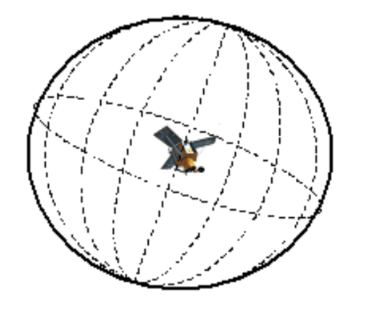
\includegraphics[width=0.7\textwidth]{img/gps_one}

        \begin{flushleft}
            if it is knows \textbf{one} $sat_i$ and the distance $d_i$ we can be in any point of the spherical surface of radius $d_i$ centered in $sat_i$.
        \end{flushleft}
    \end{minipage}
    \begin{minipage}[t]{0.3\textwidth}
        \centering
        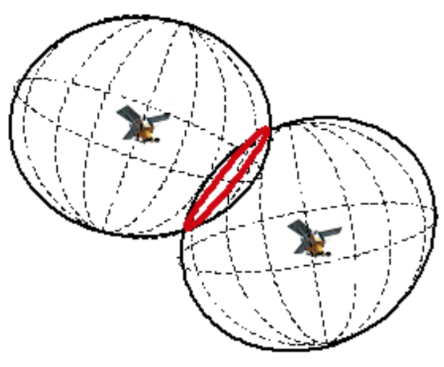
\includegraphics[width=0.7\textwidth]{img/gps_two}

        \begin{flushleft}
            if the sat known are \textbf{two} $sat_i$ and $sat_j$ both the position and the distance $d_i$, $d_j$ we can be in any point of the border given by the intersection of the two sphere's surface.
        \end{flushleft}
    \end{minipage}
    \begin{minipage}[t]{0.3\textwidth}
        \centering
        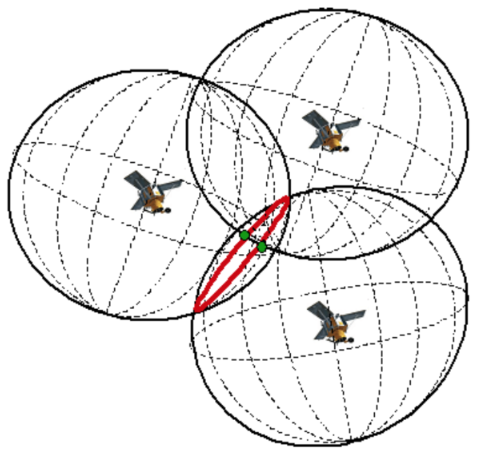
\includegraphics[width=0.7\textwidth]{img/gps_three}

        \begin{flushleft}
            adding the \textbf{third} sat, we have \textbf{three} sphere, that ends the intersection with two available points. One is on the Earth surface (us) the other is in the open space (discard).
        \end{flushleft}
    \end{minipage}
\end{figure}
In the \textbf{reality} the satellite and the receiver do not have the clock synchronize, so it is important to introduce a factor named \textit{clock error} $\Delta e$:
\begin{center}
    $d_i = \sqrt{(x_i - x_u)^2 + (y_i - y_u)^2 + (z_i - z_u)^2} + c \cdot \Delta e$
\end{center}
where:
\begin{itemize}[nosep]
    \item $x_i$, $y_i$ and $z_i$ are the sat position, \textbf{know} (NAV).
    \item $c$ is the speed of light, \textbf{know}.
    \item $x_u$, $y_u$ and $z_u$ are the position of the receiver, \textbf{unknown}.
    \item $\Delta e$ is the clock error, \textbf{unknown}.
\end{itemize}
If we consider four satellites $sat_i$, $sat_j$, $sat_k$ and $sat_p$ we end with four equations and four unknown items: $x_u$, $y_u$, $z_u$ and $\Delta e$.
\begin{center}
    \begin{math}
        \begin{cases}
            d_i = \sqrt{(x_i - x_u)^2 + (y_i - y_u)^2 + (z_i - z_u)^2} + c \cdot \Delta e \\
            d_j = \sqrt{(x_j - x_u)^2 + (y_j - y_u)^2 + (z_j - z_u)^2} + c \cdot \Delta e \\
            d_k = \sqrt{(x_k - x_u)^2 + (y_k - y_u)^2 + (z_k - z_u)^2} + c \cdot \Delta e \\
            d_p = \sqrt{(x_p - x_u)^2 + (y_p - y_u)^2 + (z_p - z_u)^2} + c \cdot \Delta e
        \end{cases}
    \end{math}
\end{center}
$\Delta e$ is equal for all satellite, because all of them are perfectly synchronize, so the \textit{clock error} is the same for each tuples (sat, recv). If recv and sat are perfectly synchronize (\textbf{time} given), with just 3 sat is possible to calculate your position. If you know where you are (\textbf{space} given), with just one sat is possible to have the clock sync, but if you do \textbf{not know} both \textbf{space} and \textbf{time} you need at least four sat to solve the equation.

\subsection{GPS limitation}
\begin{itemize}[nosep]
    \item it require a lot of power to work properly.
    \item GPS signal do not pass solid structure.
    \item affected by large buildings, unreliable in dense urban area.
    \item GPS accuracy is function of the signal reception, larger the antenna, better the signal. $miniaturization \quad \frac{1}{\alpha} \quad accuracy$
\end{itemize}

\newpage
\section{Bluetooth}
\textbf{\textit{Bluetooth}} is short-range wireless technology and it was introduce for the first time in 1994 to replace serial \textit{RS-232} wired cables. Typically used for \textbf{point-to-point} technologies. It has a coverage of 10m and creates a network named \textbf{Personal Area Network} (\textbf{PAN}), the frequency range is between $2.4GHz$ and $2.485GHz$ with few $Mbps$ of bandwidth. It is standardize in the \textit{IEEE 802.15.1} like packet-base protocol.

\begin{figure}[h]
    \centering
    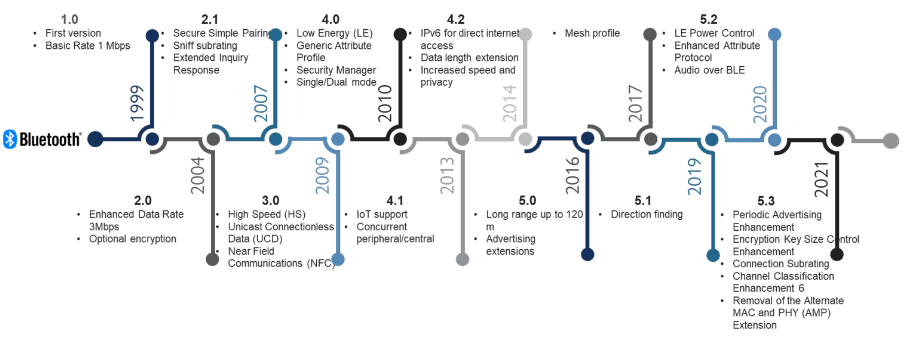
\includegraphics[width=\textwidth]{img/bluetooth_timeline}
    \caption{Bluetooth different version in the time}
\end{figure}

The bluetooth works at $2.4GHz$, like WiFi and ZigBee. A bluetooth network is named \textbf{piconet} and use a \textit{master}/\textit{slave} communication type. \\
In a bluetooth network there is always a \textbf{master} and up to seven \textbf{slave}, each slave can be only connected to one master. The master coordinates communication throughout the \textit{piconet} it can send data to every one slave connect and can request data to each slave. The slaves can only talk with the master not between them. 

\subsection{Address \& Names}
The identifier for each node into a piconet (both for slave and master) its a \textbf{unique 48 bits address}, commonly abbreviated \textbf{\textit{BD\_ADDR}}, usually is show as 12digit hexadecimal value, similar to the MAC address.
\begin{boxA}
    \textbf{Name} is pretty different, it is also possible to give to each slave an user-frendly name. It can be up to 248 bytes long and two device can share the same name.
\end{boxA}

\subsection{Connection Process}

\begin{figure}[h]
    \centering 
    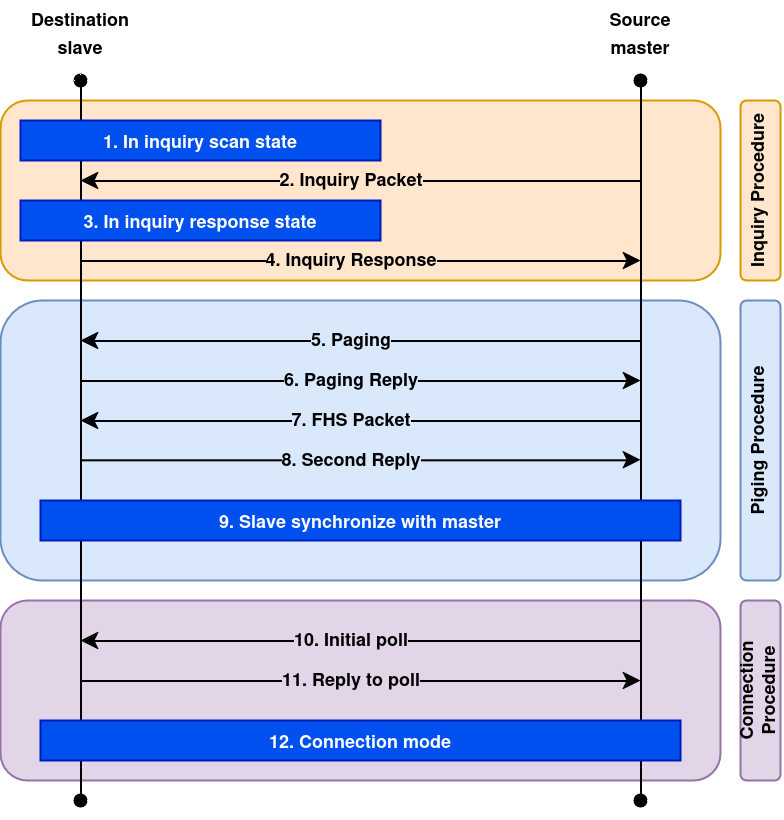
\includegraphics[width=0.75\textwidth]{img/ble_con}
    \caption{Connection Procedure in Bluetooth}
    \label{fig:ble_con}
\end{figure}

Like show in Fig.~\ref{fig:ble_con}:
\begin{itemize}[nosep]
    \item \textbf{\textit{Inquiry Procedure}}: the goal of this part is to retrive the information of each nearby nodes. A node run an inquriy scan and any listening device for this type of request, replies with its address, name and other info.
    \item \textbf{\textit{Paging Procedure}}: the purpose of this process is to create a connection between two bluetooth device. Each device \textbf{must knows} the address of the other. \textbf{\textit{FHS}}: \textbf{Frequency Hopping Sequence}.
    \item \textbf{\textit{Connection Procedure}}: after the \textit{paging} process it is necessary to define the \textbf{connection state}.
\end{itemize}

\subsection{Connection}
A bluetooth connection can have four kinds of mode:
\begin{enumerate}[nosep]
    \item \textbf{\textit{active mode}}: this is regular connected mode, where the device is actively transmitting or receiving data.
    \item \textbf{\textit{sniff mode}}: the device is active periodically for a certain amount of time (\textit{power-saving mode}).
    \item \textbf{\textit{hold mode}}: is a temporary, power-saving mode where a device sleeps for a defined period (not necessarily periodic) and then returns back to active mode when the interval passed. The master can command a slave device to hold.
    \item \textbf{\textit{park mode}}: when the master command a slave to ``park'', that slave become inactive until the master tells it to wake up.
\end{enumerate}

\subsection{Pairing}
\begin{boxA}
    Paired devices automatically establish a connection whenever thery are close enough. No UI interaction are required.
\end{boxA}
When device pair up, they share their address, name and profiles. Usually all this information are stored in memory. They also share common \textbf{secret key}, which allow them to bond whenever they want. \\
Pairing usually requires an \textbf{authentication process} where a user must validate the connection between devices, it could be different depending on the domain, some device ask to \textbf{press a button} (headset) or other can ask to \textbf{insert a code} (PC or smartphone).

\newpage
\subsection{Power Class}
The transmit power and therefore range, of a bluetooth module is defined by its \textbf{power class}. There are three defined class power:
\begin{center}
    \begin{tabular}{ | c | c | c | c | } \hline
        \textbf{Class number} & \textbf{Max Output Power}$_{dBm}$ & \textbf{Max Output Power}$_{mW}$ & \textbf{Max Range} \\ \hline
        \textbf{class 1} & 20 & 100 & 100m \\ \hline
        \textbf{class 2} & 4 & 2.5 & 10m \\ \hline
        \textbf{class 3} & 0 & 1 & 10cm \\ \hline
    \end{tabular}
\end{center}

\subsection{Profiles}
While bluetooth \textbf{specification} define how the technology \textit{works}, \textbf{profiles} define how it is \textit{used}. Two bluetooth device are \textbf{compatible} if they \textbf{support the same profiles}. Some explanation of the most common bluetooth profiles:
\begin{itemize}[nosep]
    
    \item \textbf{\textit{Serial Port Profile}} (\textbf{\textit{SPP}}): permit to substitute a serial communication protocol (like RS-232 or UART). \textit{SPP} is great for sending data between two device

    \item \textbf{\textit{Human Interface Device}} (\textbf{\textit{HID}}): is the profile to enable the receiving data from the user-input device (like mice, keyboard or joystick). \textbf{Bluetooth HID} substitute \textbf{HID} alredy defined for human input USB device, the innovation is the substitution of the USB cable for the communication.

    \item \textbf{\textit{Hands-Free Profile}} (\textbf{\textit{HFP}}) and \textbf{\textit{Headset Profile}} (\textbf{\textit{HSP}}): \textit{HFP} implements a few features on top of \textit{HSP} to allow common phone interaction (accepting/rejecting calls, etc.) that occur while the phone remains in your pocket.

    \item \textbf{\textit{Advanced Audio Distribution Profile}} (\textbf{\textit{A2DP}}): \textit{A2DP} define how audio can be transmitted from one bluetooth device to another. \textit{HFP} and \textit{HSP} have a bidiretion communication, instead \textit{A2DP} is one-way street, that permit higher quality potential.

    \item \textbf{\textit{A/V Remote Control Profile}} (\textbf{\textit{AVRCP}}): the audio/video remote control profile allows for remote controlling of a bluetooth device. It is usually implemented alongside \textit{A2DP} to allow the remote speaker to tell the audio-sending device fast-forward, rewind, etc.

\end{itemize}

\subsection{Bluetooth Stack}

\begin{figure}[h]
    \centering
    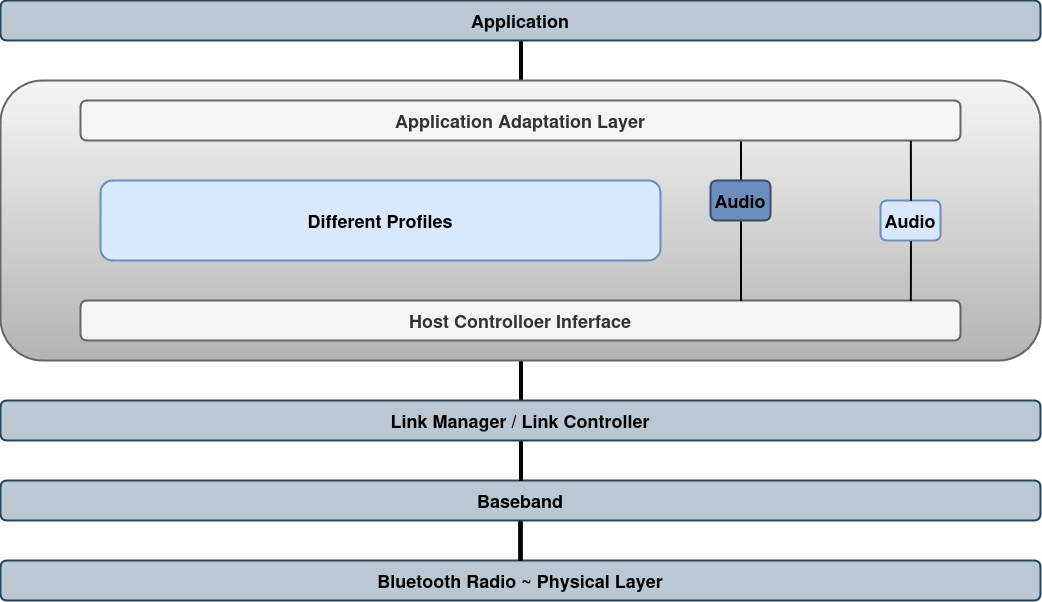
\includegraphics[width=0.85\textwidth]{img/ble_stack}
    \caption{Bluetooth Stack}
    \label{fig:ble_stack}
\end{figure}

The bluetooth protocol stack is split in two parts: a \textbf{controller stack} (in Fig.~\ref{fig:ble_stack} the blu/gray section) containing the timinig critical radio interface and \textbf{host stack} (in Fig.~\ref{fig:ble_stack} the biggest container) dealing with high level data. \\ \newline
\textbf{\textit{Radio Layer}} \\
The bluetooth radio layer is used for transmit bit from master to slave (or vice-versa) and it is similar to \textit{physical layer} in ISO/OSI model. It is a \textbf{low-power system} with 10 meters range operating in the same frequency of WiFi and ZigBee: $2.4GHz$. It defines the specification for the transceiver device:
\begin{enumerate}[nosep]
    \item \textbf{\textit{Frequency Bands and Channel Arrangement}} (\textbf{\textit{FHSS}})
    \item \textbf{Transmitter Characteristics}
    \item \textbf{Receiver Characteristics}
\end{enumerate}
The \textbf{\textit{Frequency Hopping Spread Spectrum}} is used for the transmission. The \textbf{Spectrum Spreading} is obtain by hopping between 79 frequency segments distributed between $2.402GHz$ and $2.480GHz$ ($1MHz$). The transmitter and receiver stay on one of this channels for a certain time and then hop to another channel. This system implement \textbf{Frequency Division Multiplexing} (\textbf{FDM}) and \textbf{Time Division Multiplexing}

\begin{figure}[h]
    \centering
    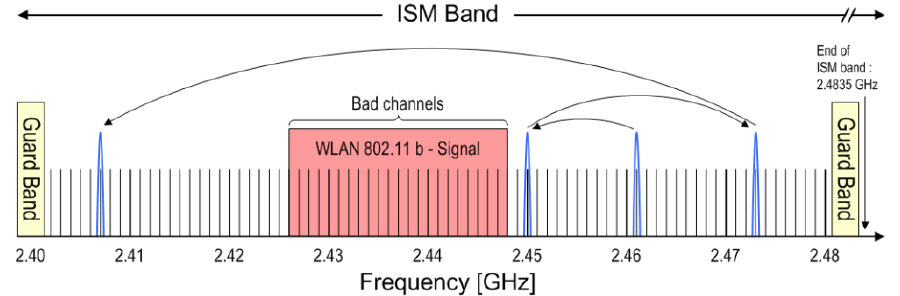
\includegraphics[width=0.75\textwidth]{img/ble_fhss}
    \caption{Frequency Hopping Spread Spectrum}
\end{figure}
The changes of frequency it could be performed in two different way:

\begin{figure}[h]
    \centering
    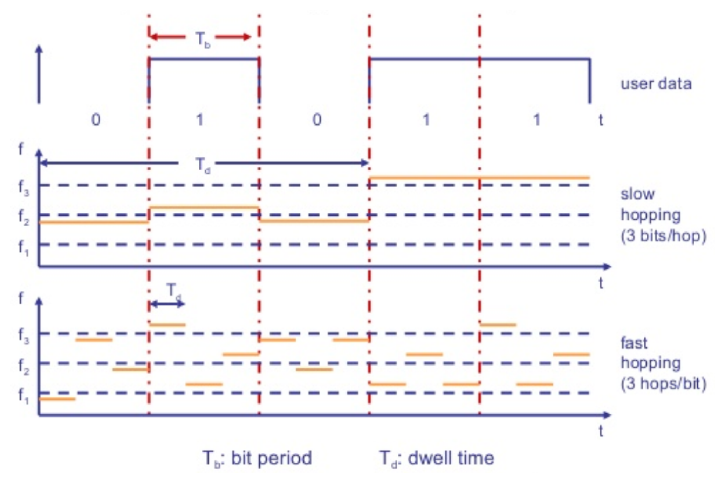
\includegraphics[width=0.75\textwidth]{img/ble_hop}
\end{figure}
\begin{itemize}[nosep]
    
    \item \textbf{\textit{slow hopping}}: the transmitter uses one frequency for several bit period:
    \begin{itemize}[nosep]
        \item typically cheaper (relaxed sync constraints, more time per slot)
        \item not immune to narrowband interferances
    \end{itemize}
    
    \item \textbf{\textit{fast hopping}}: the transmitter uses several frequencies for one period:
    \begin{itemize}[nosep]
        \item typically expensive (hard sync constraints, more slot jumps and high resync frequency)
        \item almost immune to narrowband
        \item rate 1600 hops/sec: $625 \mu s$ of slot time
    \end{itemize}

\end{itemize}
\textbf{\textit{Baseband Layer}} \\
While the \textbf{radio layer} is controlled by the transceiver, the \textbf{baseband layer} is implemented by the controller of a device how want to transmit in bluetooth. The \textit{baseband} is the \textbf{physical layer} of the bluetooth and is used to manages physical channel and links, but also \textit{error connection}, \textit{data whitening}, \textit{hop selection} and \textit{bluetooth security}. \\
Is is used to managed \textbf{synchronous} and \textbf{asynchronous} links. It handles packet and perform the \textit{inquiry} and the \textit{paging} for create connection with nearby device. The baseband layer applies a \textbf{time division duplex} (\textbf{TDD}) scheme to alternating transmitter and receiver. Baseband handles two types of links:
\begin{enumerate}[nosep]
    \item \textbf{\textit{Synchronous Connection Oriented}} link (\textbf{\textit{SCO}}): is a symmectric point-to-point link between a master and a single slave in the piconet. The master maintains the \textit{SCO} link by using reserved slot at regular intervals:
    \begin{itemize}[nosep]
        \item \textit{SCO} is commonly used for the transmission of voice information.
        \item master can support up to three simultaneously \textit{SCO} links, instead, slave only two (sometimes three).
        \item \textit{SCO} packets are never re-transmitted, normally used for $64kB/s$ speech transmission.
    \end{itemize}
    \item \textbf{\textit{Asynchronous Connection Less}} link (\textbf{\textit{ACL}}): is point-to-multipoint between the master and all the slave present in the piconet. In the slot not reserved for the \textit{SCO} links, the master can establish an \textit{ACL} link to any slave
    \begin{itemize}[nosep]
        \item slave alredy into a \textit{SCO} communication are included.
        \item only a single \textit{ACL} link can exist.
        \item for most of \textit{ACL} packets, re-transmission is applied.
    \end{itemize}
\end{enumerate}
These means that \textit{SCO} does not need a connection, there is not an acknoledgement (like \textbf{UDP}), instead the \textit{ACL} need the \textit{ACK} to check if the message needs to be re-transmitted (like \textbf{TCP}). \\
\textbf{\textit{Bluetooth Packet}}
\begin{center}
    \begin{tabular}{ | c | c | c | c | } \hline
        \textbf{bits} & 72 & 54 & 0 - 2745 \\ \hline
        \textbf{description} & \textbf{access code} & \textbf{header} & \textbf{payload} \\ \hline
    \end{tabular}
\end{center}
\begin{enumerate}[nosep]
    \item \textbf{\textit{access code}}: is used for \textit{time synchronization}, \textit{offset compensation}, \textit{paging} and \textit{inquiry}.
    \item \textbf{\textit{header}}: contains information for \textit{packet acknoledgement}, \textit{packet numbering} for out-of-order packet reordering, \textit{flow control}, \textit{slave address} and \textit{error check} for header.
    \item \textbf{\textit{payload}}: can contain either voice field, data field or both. The payload will also contain a \textbf{payload header}.
\end{enumerate}
\textbf{\textit{Other Baseband Function}} \\
The baseband makes other features available like:
\begin{enumerate}[nosep]
    \item \textbf{\textit{error correction}}:
    \begin{itemize}[nosep]
        \item $\frac{1}{3}$ \textbf{rate FEC} (\textbf{Forward Error Correction}): every bit is repeated three times (\textbf{rendundancy}), in this way the receiver can discard up to two bits and validate the transmission.
        \item $\frac{2}{3}$ \textbf{rate FEC}: it use a \textit{polynomial generator} to \textbf{encode} ten bits code into fiftheen bits code.
        \begin{boxA}
            If i want to send $1010001111$ that is ten bits long, i divide into two pieces: $10100$ and $01111$ and i will compute the XOR: $10100 \oplus 01111 = 11011$. I will send the three concatenated values: $m = [10100, 01111, 11011]$. The receiver it could receive wrong the second value, but it can rebuild it performing the XOR between the first and third value. It allow only one ``wrong'' value, if not it can not reconstruct the original message.
        \end{boxA}
        \item \textbf{ARQ scheme} (\textbf{Automatic Repeat Request}): uses \textit{ACK}, \textit{NACK}, \textit{RTO}, etc.
    \end{itemize}
    \item \textbf{\textit{flow control}}: use \textbf{FIFO} queues both in \textit{ACL} and \textit{SCO} links for transmission and receive. In the case that the \textbf{RX FIFO} queues are full, \textbf{flow control} is used to avoid \textbf{congestion} and \textbf{packet drop}. The receiver send a \textbf{stop} indication, the transmitter \textbf{blocks} its \textbf{TX FIFO} queues. When the queues of the receiver are ready it sends an \textbf{go} signal to resume the transmission.
    \item \textbf{\textit{synchronization}}: the piconet is sync using the master clock and it is needed for the transmission at least three information:
    \begin{itemize}[nosep]
        \item \textbf{channel hopping sequence}
        \item \textbf{phase of the sequence}
        \item \textbf{channel access code} to place on the packets (piconet code)
    \end{itemize}
    \item \textbf{\textit{security}}: at link layer, security is maintained by authentication of the peers and encryption of the information. For this basic security we need a public address which is unique for each device, two secret key (authentication keys and encryption keys) and a random number generator.
\end{enumerate}
\textbf{\textit{Link Manager Layer}} \\
On top that layer it is used the \textbf{\textit{Link Manager Protocol}} (\textbf{\textit{LMP}}) that carries out link setup, authentication, link configuration and other protocol. The Link-Controller/Baseband provides services to \textbf{LMP} likes: \textit{authentication}, \textit{pairing}, \textit{encryption}, \textit{change link key}, \textit{slot/clock offset request}, \textit{switch master/slave role}, \textit{hold/sniff/park role} and \textit{quality of service}. \\
\textbf{\textit{Automotive \& Bluetooth}}:
\begin{itemize}[nosep]
    \item \textbf{in-car infortainment system}: permit hands-free audio, calling and application control.
    \item \textbf{remote keyless system}: smart phone are the new key, that use \textit{proximity detection} for locking and unlocking car.
    \item \textbf{in-vehicle wearables}: permit to monitoring the driver health.
    \item \textbf{under-the-hood \& connected maintenance}: allow to transfer diagnostic information.
\end{itemize}
\begin{center}
    \begin{tabular}{ | c | c | c | } \hline
        & \textbf{bluetooth} & \textbf{bluetooth low energy} \\ \hline
        \textbf{freq. band} & $2.4GHz$ ISM Band & $2.4GHz$ ISM Band \\ \hline
        \textbf{no. of channel} & 79, one $1MHz$ & 40, one $2MHz$ \\ \hline
        \textbf{power consumption} & low & less \\ \hline
        \textbf{data rate} & between $1Mbps$ and $3Mbps$ & $1Mbps$ \\ \hline
        \textbf{latency} & $\approxeq$ 100ms & $\approxeq$ 6ms \\ \hline
        \textbf{range} & < 30m & 50m (in open area: 150m) \\ \hline
        \textbf{topology} & peer-to-peer (1:1) & \begin{tabular}{@{}c@{}}peer-to-peer (1:1) \\ star (many:1) \\ broadcast (1:many) \\ mesh (many:many) \end{tabular} \\ \hline
        \textbf{device pairing} & required & not required \\ \hline
        \textbf{voice capable} & yes & no \\ \hline
        \textbf{node/active slave} & 7 & unlimited \\ \hline
        \textbf{security} & 64bits or 128 bits & 128 bits AES \\ \hline
        \textbf{smartphone compatibility} & 100\% & 100\% \\ \hline
        \textbf{use cases} & 
        \begin{tabular}{@{}c@{}}
            streaming application \\ 
            like audio streaming, \\ 
            file transfer and
            \\ headset 
        \end{tabular} & 
        \begin{tabular}{@{}c@{}}
            location beacons, \\ 
            smart home application, \\ 
            medical deivces, \\ 
            industrial monitoring \\ 
            and fitness trackers 
        \end{tabular} \\ \hline
    \end{tabular}
\end{center}

\newpage
\section{LoRa: Long Range}

\begin{figure}[h]
    \centering
    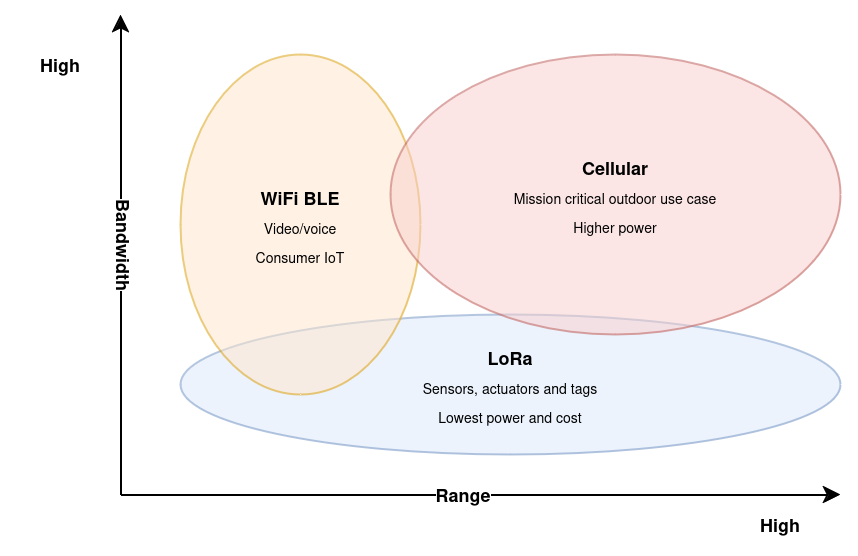
\includegraphics[width=0.5\textwidth]{img/lora}
\end{figure}
\textbf{LoRa} has an unlicenced frequency band equal to: $868MHz$ (in Europe) and very long range coverage: up to \textbf{10 km}. It is composed by two part:
\begin{enumerate}[nosep]
    \item \textbf{LoRa}: the \textit{physical layer} that is \textbf{proprietary}.
    \item \textbf{LoRaWAN}: \textbf{Long Range Wide Area Network} that defines the upper layers (in particular MAC layer).
\end{enumerate}

\newpage
\subsection{LoRa Stack}

\begin{figure}[h]
    \centering
    \begin{minipage}[t]{0.3\textwidth}
        \centering
        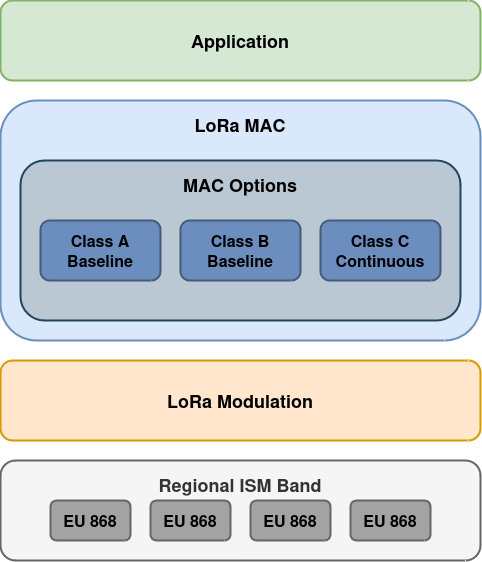
\includegraphics[width=\textwidth]{img/lora_stack}
        \caption{LoRa Stack}
    \end{minipage}
    \begin{minipage}[t]{0.65\textwidth}
        \centering
        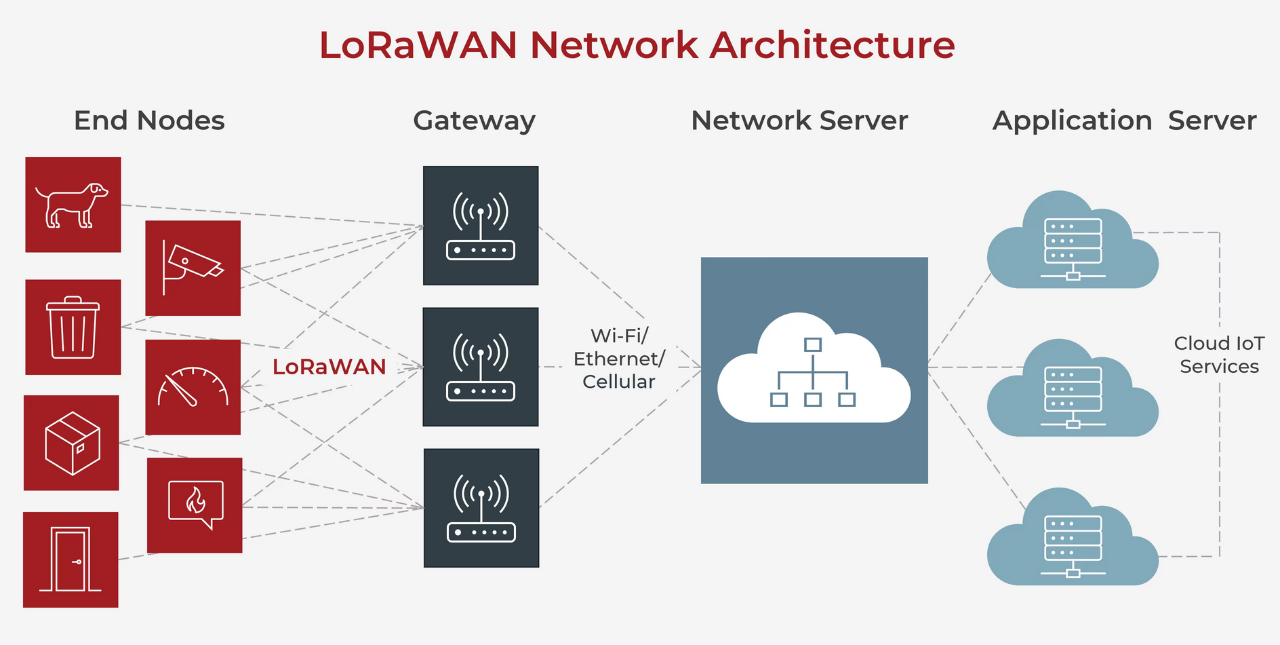
\includegraphics[width=\textwidth]{img/lora_network}
        \caption {LoRaWAN network architecture}
        \label{fig:lora_net}
    \end{minipage}
\end{figure}
\textbf{LoRaWan} defines the \textit{MAC Layer}, the point-to-point network, the communication protocol and the system architecture standard (Fig. \ref{fig:lora_net}). It, also, managed the \textit{frequency}, \textit{data rate} and \textit{power device}.
\begin{itemize}[nosep]
    \item \textbf{end device, node} an embedded object with low-power communication constraints.
    \item \textbf{gateway} receive broadcast data and send data from/to the \textit{end device}.
    \item \textbf{network server} route message from \textit{end device} to the right application, and back.
\end{itemize}
\textbf{\textit{Addressing}}: to each \textit{device} is assign an \textbf{unique identifier} (\textbf{DevEUI}) of 64 bits, instead to each \textit{application} is attribute \textbf{distinctive fingerprint} (\textbf{AppEUI}) of 64 bits, moreover after the access inside a network of a new device it receives a \textbf{dynamic} \textit{non-unique} address of 32 bits (\textbf{DevAddr}). \\ \newline
\textbf{\textit{Frame Counter}} prevent \textbf{replay attack}, to prevent this each nodes (both \textit{end device} and \textit{server}) reject message that contain frame counter that is lower than the expected ones.

\newpage
The \textit{end device} could be classified into \textbf{three different classes}:
\begin{figure}[h]
    \centering
    \begin{minipage}[t]{0.45\textwidth}
        \centering
        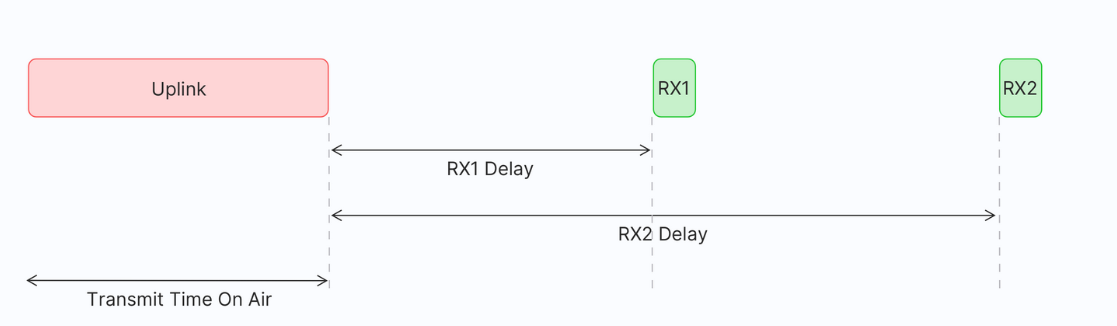
\includegraphics[width=\textwidth]{img/lora_classA}
        \caption{\textbf{Class A}}

        \begin{flushleft}
            Support bidirectional communication (from/to gateway), transmission messages can be sent in any time (random), two possible receive windows at specific time (after 1s and after 2s) after a transmission message, the gateway can reply in one of this two windows.
        \end{flushleft}
    \end{minipage}
    \begin{minipage}[t]{0.45\textwidth}
        \centering
        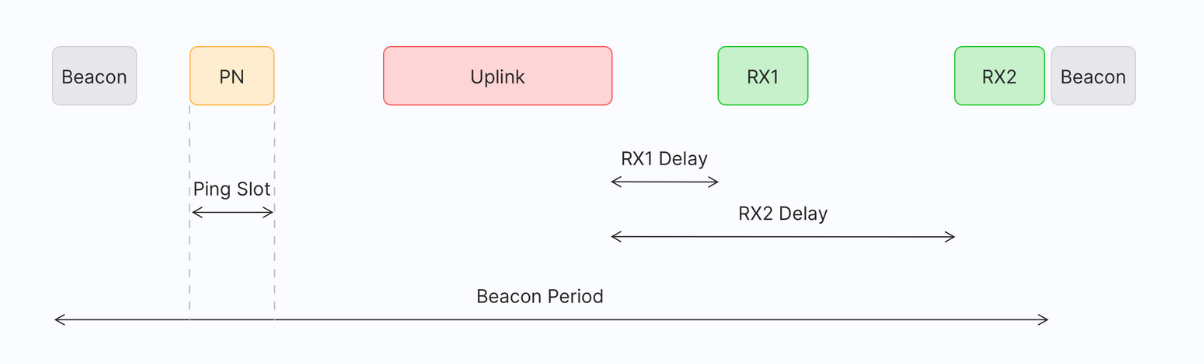
\includegraphics[width=\textwidth]{img/lora_classB}
        \caption{\textbf{Class B}}

        \begin{flushleft}
            Extend \textit{class A} by adding scheduled receive windows for receiving message from the gateway/server. It use time-sync beacons transmitted by the gateway, the \textit{end device} periodically open receive window.
        \end{flushleft}
    \end{minipage}
\end{figure}

\begin{figure}[h]
    \centering
    \begin{minipage}[t]{0.45\textwidth}
        \centering
        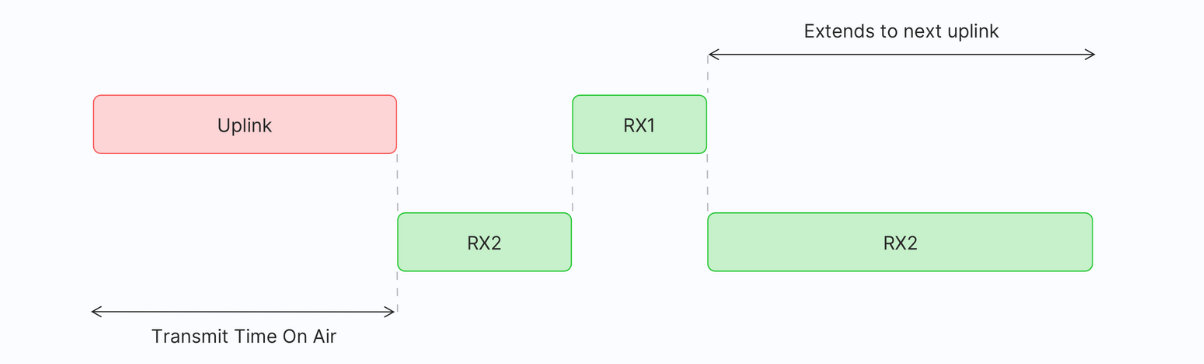
\includegraphics[width=\textwidth]{img/lora_classC}
        \caption{\textbf{Class C}}

        \begin{flushleft}
            Extend \textit{class A} by keeping the receive window open unless they are transmitting. This allow \textbf{low latency} communication, but it consume more energy than \textit{class A} device.
        \end{flushleft}
    \end{minipage}
\end{figure}

\subsection{Secuirty}
LoRaWAN specifies three different class of \textbf{security keys}: \textbf{\textit{NwSKey}}, \textbf{\textit{AppSKey}} and \textbf{\textit{AppKey}}, all have the lenght of 128 bits. The algorithm use for the encryption is \textbf{\textit{AES-128}}. \\
When a device joins the network (called \textbf{activation} or \textbf{join}), an \textit{application session key} (\textbf{AppSKey}) and \textit{network session key} (\textbf{NwSKey}) are generated that will be used for the duration of the session. The \textbf{AppSKey} is the \textit{private key}, instead the \textbf{NwSKey} is the \textit{public key}. The \textbf{Network Session Key} is used for the interaction between the node and the server and it is used to validate the integrity of each message using the \textbf{Message Integrity Code} (\textbf{MIC}). The \textbf{MIC} is similar to checksum expect that it prevents intentional tampering with message (\textbf{AES-CMAC}), it is also used to map the \textbf{DevAddr} to both \textbf{AppEUI} and \textbf{DevEUI}. The \textbf{Application Session Key} is used for encryption and decryption of the payload. \\
The \textbf{Application Key} (\textbf{AppKey}) is only know by the device and the application. The \textbf{NwSKey} and \textbf{AppSKey} are derived from this key. If you dinamically activate the device (\textbf{Over the Air Activation - OTAA}) the two sessione key are regenerate.

\subsection{MAC Commands}
The \textit{end device} and the \textit{server} use \textbf{MAC Commands} for configure the transmission and for the communication.
\begin{itemize}[nosep]
    \item checking connectivity
    \item requesting the status of the device
    \item adapting the data rate of the device
    \item modify channel settings
\end{itemize}

\begin{center}
    \begin{tabular}{ | c | c | } \hline
        \textcolor{green}{\textbf{Pros}} & \textcolor{red}{\textbf{Cons}} \\ \hline
        long range & not realtime data (packet each minutes) \\ \hline
        low power & not use for domotic house (ZigBee or Bluetooth) \\ \hline
        \begin{tabular}{@{}c@{}}
            low cost \\ 
            $\approxeq$ 20\$ per node
        \end{tabular} & watch video (WiFi) \\ \hline
        \begin{tabular}{@{}c@{}}
            low bandwidth \\ 
            between $250bit/s$ and $11kbit/s$
        \end{tabular} & \\ \hline
        \begin{tabular}{@{}c@{}}
            secure: 128 bits \\ 
            end-to-end encryption
        \end{tabular} & \\ \hline
    \end{tabular}
\end{center}